
\chapter{Variable-speed motor controls}

An alternative to control valves for adjusting fluid flow is to regulate the speed of the machine(s) motivating fluid to flow.  In the case of liquid flow control, this would take the form of variable-speed pumps.  In the case of gas flow control, it would mean varying the rotational speed of compressors or blowers.

Flow control by machine speed control makes a lot of sense for some process applications.  It is certainly more energy-efficient\footnote{Regulating fluid flow by using a throttling valve along with a constant-speed pump is analogous to regulating an automobile's speed by applying varying force to the brake pedal while holding the accelerator pedal at its full-power position!} to vary the speed of the machine pushing fluid to control flow, as opposed to letting the machine run at full speed all the time and adjusting flow rate by throttling the machine's discharge (outlet) or recycling fluid back to the machine's suction (inlet).  The fact that the system has one less component in it (no control valve) also reduces capital investment and potentially increases system reliability:

$$\includegraphics{motor_01.eps}$$

Modern power electronics provide the means to electronically control the speed of almost any type and size of electric motor, using a device called a motor \textit{drive}.  DC motor drives vary voltage and current to the armature and field windings of the motor.  In general, DC motor speed is directly proportional to armature voltage, and inversely proportional to field current.  AC motor drives vary the \textit{frequency}\footnote{AC drives also vary the amount of voltage applied to the motor along with frequency, but this of secondary importance to the varying of frequency to control speed.} of the power applied to the motor's stator windings, because frequency is what establishes the speed of the stator's rotating magnetic field which the rotor follows.  \index{Motor drive}  \index{Drive, electric motor}

DC motors were once considered clearly superior to AC motors in variable-speed applications where high starting torque (torque generated at zero speed) was needed.  The advent of sophisticated variable-frequency drive (VFD) electronics, however, greatly expanded the useful operating speed range of AC induction motors to the point where one can do almost any task\footnote{This includes using an AC induction motor as a \textit{servo} for precise positioning control!} with an AC motor that used to be possible only with a DC motor.  This is highly advantageous, because AC induction motors are much simpler and more reliable machines than DC motors.  DC motors use commutators and brushes to conduct electrical power to their rotating armatures, both of these components being subject to wear.  AC induction motors convey power to their rotors by electromagnetic induction, not by direct contact, and so neither commutators nor brushes are necessary.  In fact, the only ``wearing'' component in an AC induction motor are the bearings holding the shaft, which of course are common to \textit{all} rotating machines and therefore not a liability peculiar to AC induction motors.  \index{Variable-frequency drive}  \index{VFD}

\vskip 10pt

Further advantages of electric motor speed control, whether DC or AC, include the ability to ``soft-start'' the machine instead of always accelerating rapidly from a full stop to full speed.  Soft-starting electric motors greatly reduces the wear on machines, increasing their service life.  In applications such as conveyor belt control, robotic machine motion control, and electric vehicle propulsion, variable-speed motor technology makes perfect sense as a control mechanism because the prime mover device is already (in most cases) an electric motor, with precise speed control of that motor yielding many practical benefits.  In some applications, \textit{regenerative braking} may be possible: where the motor is used as an electrical generator to slow down the machine on command.  Regenerative braking transfers kinetic energy within the machine back to the power grid where it may be productively used in other processes, saving energy and reducing wear on any mechanical (friction) brakes already installed in the machine.

\vskip 10pt

With all these advantages inherent to variable-speed pumps, fans, and compressors (as opposed to using dissipative control valves), one might wonder, ``Why would anyone \textit{ever} use a control valve to regulate flow?  Why not control \textit{all} fluid flows using variable-speed pumping machines?''  Several good answers exist to this question:

\begin{itemize}
\item Variable-speed machines often cannot increase or decrease fluid flow rates as rapidly as control valves
\item Control valves have the ability to positively halt flow; a stopped pump or blower will not necessarily prevent flow from going through
\item Some process applications \textit{must} contain a dissipative element in order for the system to function (e.g. let-down valves in closed-loop refrigeration systems)
\item Split-ranging may be difficult or impossible to achieve with multiple machine speed control
\item Limited options for fail-safe status
\item In many cases, there is no machine dedicated to a particular flow path (e.g. a pressure release valve, or a valve controlling water flow from a dam) for us to control the speed of
\end{itemize}













\filbreak
\section{DC motor speed control}

DC electric motors generate torque by a reaction between two magnetic fields: one field established by stationary ``field'' windings (coils), and the other by windings in the rotating armature.  Some DC motors lack field windings, substituting large permanent magnets in their place so that the stationary magnetic field is constant for all operating conditions.  

In any case, the operating principle of a DC electric motor is that current passed through the armature creates a magnetic field that tries to align with the stationary magnetic field.  This causes the armature to rotate:

$$\includegraphics{motor_16.eps}$$

However, a set of segmented copper strips called a \textit{commutator} breaks electrical contact with the now-aligned coil and energizes another coil (or in the simple example shown above, it re-energizes the same loop of wire in the opposite direction) to create another out-of-alignment magnetic field that continues to rotate the armature.  Electrical contact between the rotating commutator segments and the stationary power source is made through carbon \textit{brushes}.  These brushes wear over time (as does the commutator itself), and must be periodically replaced.  \index{Commutator, DC motor}  \index{Brush, DC motor}

\filbreak

Most industrial DC motors are built with multiple armature coils, not just one as shown in the simplified illustration above.  A photograph of a large (1250 horsepower) DC motor used to propel a ferry ship is shown here, with the field and armature poles clearly seen (appearing much like spokes in a wheel):

$$\includegraphics[width=4in]{motor_23.eps}$$

A close-up of one brush assembly on this large motor shows both the carbon brush, the brush's spring-loaded holder, and the myriad of commutator bars the brush makes contact with as the armature rotates:

$$\includegraphics[width=4in]{motor_24.eps}$$

DC motors exhibit the following relationships between mechanical and electrical quantities:

\vskip 10pt

\noindent
\textbf{Torque:}

\begin{itemize}
\item Torque is directly proportional to armature magnetic field strength, which in turn is directly proportional to current through the armature windings
\item Torque is also directly proportional to the stationary pole magnetic field strength, which in turn is directly proportional to current through the field windings (in a motor with non-permanent field magnets)
\end{itemize}

\noindent
\textbf{Speed:}

\begin{itemize}
\item Speed is limited by the counter-EMF generated by the armature as it spins through the stationary magnetic field.  This counter-EMF is directly proportional to armature speed, and also directly proportional to stationary pole magnetic field strength (which is directly proportional to field winding current in a motor that is not permanent-magnet)
\item Thus, speed is directly proportional to armature voltage
\item Speed is also inversely proportional to stationary magnetic field strength, which is directly proportional to current through the field windings (in a motor with non-permanent field magnets)
\end{itemize}

A very simple method for controlling the speed and torque characteristics of a wound-field (non-permanent magnet) DC motor is to control the amount of current through the field winding:

$$\includegraphics{motor_17.eps}$$

Decreasing the field control resistor's resistance allows more current through the field winding, strengthening its magnetic field.  This will have two effects on the motor's operation: first, the motor will generate more torque than it did before (for the same amount of armature current) because there is now a stronger magnetic field for the armature to react against; second, the motor's speed will decrease because more counter-EMF will be generated by the spinning armature for the same rotational speed, and this counter-EMF naturally attempts to equalize with the applied DC source voltage.  Conversely, we may increase a DC motor's speed (and reduce its torque output) by increasing the field control resistor's resistance, weakening the stationary magnetic field through which the armature spins. 

Regulating field current may alter the balance between speed and torque, but it does little to control total motor \textit{power}.  In order to control the power output of a DC motor, we must also regulate armature voltage and current.  Variable resistors may also be used for this task, but this is generally frowned upon in modern times because of the wasted power.  

\filbreak

A better solution is to have an electronic power control circuit very rapidly switch transistors on and off, switching power to the motor armature.   This is called \textit{pulse-width modulation}, or \textit{PWM}.  \index{Pulse width modulation}  \index{PWM}

$$\includegraphics{motor_18.eps}$$

The \textit{duty cycle} (on time versus on+off time) of the pulse waveform will determine the fraction of total power delivered to the motor:

$$\includegraphics{motor_19.eps}$$

Such an electronic power-control circuit is generally referred to as a \textit{drive}.  Thus, a \textit{variable-speed drive} or \textit{VSD} is a high-power circuit used to control the speed of a DC motor.  Motor drives may be manually set to run a motor at a set speed, or accept an electronic control signal to vary the motor speed in the same manner an electronic signal commands a control valve to move.  When equipped with remote control signaling, a motor drive functions just like any other final control element: following the command of a process controller in order to stabilize some process variable at setpoint.  \index{Variable-speed drive}  \index{VSD}

\filbreak

An older technology for pulsing power to a DC motor is to use a \textit{controlled rectifier} circuit, using SCRs instead of regular rectifying diodes to convert AC to DC.  Since the main power source of most industrial DC motors is AC anyway, and that AC must be converted into DC at some point in the system, it makes sense to integrate control right at the point of rectification:  \index{Controlled rectifier}  \index{Rectifier, SCR controlled}

$$\includegraphics{motor_20.eps}$$

Controlled rectifier circuits work on the principle of varying the ``trigger'' pulse times relative to the AC waveform pulses.  The earlier the AC cycle each SCR is triggered on, the longer it will be on to pass current to the motor.  The ``phase control'' circuitry manages all this pulse timing and generation.

\filbreak

A DC motor drive that simply varied power to the motor according to a control signal would be crude and difficult to apply to the control of most processes.  What is ideally desired from a variable-speed drive is precise command over the motor's \textit{speed}.  For this reason, most VSDs are designed to receive feedback from a tachometer mechanically connected to the motor shaft, so the VSD ``knows'' how fast the motor is turning.  The tachometer is typically a small DC generator, producing a DC voltage directly proportional to its shaft speed (0 to 10 volts is a common scale).  With this information, the VSD may throttle electrical power to the motor as necessary to achieve whatever speed is being commanded by the control signal.  Having a speed-control feedback loop built into the drive makes the VSD a ``slave controller'' in a cascade control system, the drive receiving a speed setpoint signal from whatever process controller is sending an output signal to it:

$$\includegraphics{motor_26.eps}$$

\filbreak

A photograph of the tachogenerators (dual, for redundancy) mechanically coupled to that large 1250 horsepower ferry ship propulsion motor appears here:

$$\includegraphics[width=3in]{motor_27.eps}$$

The SCRs switching power to this motor may be seen here, connected via twisted-pair wires to control boards issuing ``firing'' pulses to each SCR at the appropriate times:

$$\includegraphics[width=3in]{motor_28.eps}$$

The integrity of the tachogenerator feedback signal to the VSD is extremely important for safety reasons.  If the tachogenerator becomes disconnected -- whether mechanically or electrically (it doesn't matter) -- from the drive, the drive will ``think'' the motor is not turning.  In its capacity as a speed \textit{controller}, the drive will then send full power to the DC motor in an attempt to get it up to speed.  Thus, loss of tachogenerator feedback causes the motor to immediately ``run away'' to full speed.  This is undesirable at best, and likely dangerous in the case of motors as large as the one powering this ship.

\vskip 10pt

As with all forms of electric power control based on pulse durations and duty cycles, there is a lot of electrical ``noise'' broadcast by VSD circuits.  Square-edged pulse waveforms created by the rapid on-and-off switching of the semiconductor power devices are equivalent to infinite series of high-frequency sine waves\footnote{This equivalence was mathematically proven by Jean Baptiste Joseph Fourier (1768-1830), and is known as a \textit{Fourier series}.}, some of which may be of high enough frequency to self-propagate through space as electromagnetic waves.  This \textit{radio-frequency interference} or \textit{RFI} may be quite severe given the high power levels of industrial motor drive circuits.  For this reason, it is \textit{imperative} that neither the motor power conductors nor the conductors feeding AC power to the drive circuit be routed anywhere near small-signal or control wiring, because the induced noise \textit{will} wreak havoc with whatever systems utilize those low-level signals.  \index{Radio frequency interference from motor drive circuits}  \index{RFI}  \index{Fourier, Jean Baptiste Joseph}  \index{Fourier series}

RFI noise on the AC power conductors may be reduced by routing the AC power through low-pass filter circuits called \textit{line reactors} placed near the drive.  These line reactors, consisting of ferrous metal core inductors wired in series with the drive, block high-frequency noise from propagating back to the rest of the AC power distribution wiring where it may influence other electronic equipment.  However, there is little that may be done about the RFI noise between the drive and the motor other than to shield the conductors inside of well-grounded metallic conduit and/or to use grounded-shield power cables.  \index{Line reactor}












\filbreak
\section{AC motor speed control}

AC induction motors are based on the principle of a \textit{rotating magnetic field} produced by a set of stationary windings (called \textit{stator} windings) energized by AC power of different phases.  The effect is not unlike a series of blinking ``chaser'' light bulbs which appear to ``move'' in one direction due to the blinking sequence.  If sets of wire coils (windings) are energized in a like manner -- each coil reaching its peak field strength at a different time from its adjacent neighbor -- the effect will be a magnetic field that ``appears'' to move in one direction.  If these windings are oriented around the circumference of a circle, the moving magnetic field rotates about the center of the circle, as illustrated by this sequence of images (read left-to-right, top-to-bottom, as if you were reading words in a sentence):   \index{Rotating magnetic field}  \index{Stator}

$$\includegraphics[width=1in]{03232x01.eps} \hskip 20pt \includegraphics[width=1in]{03232x02.eps} \hskip 20pt \includegraphics[width=1in]{03232x03.eps} \hskip 20pt \includegraphics[width=1in]{03232x04.eps}$$

$$\includegraphics[width=1in]{03232x05.eps} \hskip 20pt \includegraphics[width=1in]{03232x06.eps} \hskip 20pt \includegraphics[width=1in]{03232x07.eps} \hskip 20pt \includegraphics[width=1in]{03232x08.eps}$$

$$\includegraphics[width=1in]{03232x09.eps} \hskip 20pt \includegraphics[width=1in]{03232x10.eps} \hskip 20pt \includegraphics[width=1in]{03232x11.eps} \hskip 20pt \includegraphics[width=1in]{03232x12.eps}$$

To view a flip-book animation of this same sequence, turn to Appendix \ref{animation_3phase_motor} beginning on page \pageref{animation_3phase_motor}.

Any magnetized object placed in the center of this circle will attempt to spin at the same rotational speed as the rotating magnetic field.  \textit{Synchronous} AC motors use this principle, where a magnetized rotor precisely follows the magnetic field's speed.  \index{Synchronous motor}

Any electrically conductive object placed in the center of the circle will experience \textit{induction} as the magnetic field direction changes around the conductor.  This will induce electric currents within the conductive object, which in turn will react against the rotating magnetic field in such a way that the object will be ``dragged along'' by the field, always lagging a bit in speed.  \textit{Induction} AC motors use this principle, where a non-magnetized (but electrically conductive) rotor rotates at a speed slightly less\footnote{The difference between the synchronous speed and the rotor's actual speed is called the motor's \textit{slip speed}.} than the synchronous speed of the rotating magnetic field.  \index{Induction motor}  \index{Synchronous speed}  \index{Slip speed}

\filbreak

The rotational speed of this magnetic field is directly proportional to the frequency of the AC power, and inversely proportional to the number of poles in the stator:

$$S = {120 f \over n}$$

\noindent
Where,

$S$ = Synchronous speed of rotating magnetic field, in revolutions per minute (RPM)

$f$ = Frequency, in cycles per second (Hz)

$n$ = Total number of stator poles per phase (the simplest possible AC induction motor design will have two poles)

\vskip 10pt

The relationship between synchronous speed, frequency, and pole number may be understood by analogy: the speed at which the lights in a ``chaser'' light array appear to move is a function of the blinking frequency and the number of light bulbs per unit length.  If the number of light bulbs in such an array is doubled by placing additional bulbs between the existing bulbs (so as to maintain the same array length), the apparent speed will be cut in half: with less distance between each pair of bulbs, it takes more cycles (more ``blinks'') for the sequence to travel the entire length of the array.  Likewise, an AC stator with more poles in its circumference will require more cycles of AC power for the rotating magnetic field to complete one revolution.

A \textit{synchronous} AC motor will spin at the exact same speed as the rotating magnetic field: a practical example is a 4-pole synchronous motor spinning at 1800 RPM with an applied power frequency of 60 Hz.  An \textit{induction} AC motor will spin at slightly less than the speed of the magnetic field: a practical example is a 4-pole induction motor spinning at 1720 RPM with an applied power frequency of 60 Hz (i.e. 80 RPM ``slip'' speed).  Induction motors are simpler both in construction and operation, making them the most popular of the two types of AC electric motors in industry.  \index{Slip speed}

\vskip 10pt

While the number of poles in the motor's stator is a quantity fixed\footnote{Multi-speed motors do exist, with selectable pole configurations.  An example of this is an electric motor with extra sets of stator windings, which may be connected to form a 4-pole configuration for high speed, and an 8-pole configuration for low speed.  If the normal full-load ``high'' speed for this motor is 1740 RPM, the normal full-load ``low'' speed will be approximately half that, or 870 RPM.  Given a fixed line frequency, this motor will only have these two speeds to choose from.} at the time of the motor's manufacture, the frequency of power we apply may be adjusted with the proper electronic circuitry.  A high-power circuit designed to produce varying frequencies for an AC motor to run on is called a \textit{variable-frequency drive}, or \textit{VFD}.  \index{Variable-frequency drive}  \index{VFD}

Variable-frequency motor drives are incredibly useful devices, as they allow what would normally be a fixed-speed electric motor to provide useful power over a wide range of speeds.  The benefits of variable-speed operation include reduced power consumption (only spinning the motor as fast as it needs to move, and no faster), reduced vibration (less speed = reduced vibrational forces), and the ability to ramp the motor's speed up and down for reduced wear and tear on mechanical components resulting from acceleration forces.

\vskip 10pt

Another feature common to most VFDs is the ability to actively \textit{brake} the load.  This is when the drive causes the motor to actively apply a negative torque to the load to slow it down.  Some VFDs even provide means to recover the kinetic energy of the load during the braking process, resulting in further energy savings.

\filbreak

Variable-frequency AC motor drives consist of electronic components to convert the constant-frequency AC input power into variable-frequency (and variable-voltage) AC output power for the motor to run on.  This usually takes place in three distinct sections.  The \textit{rectifier} section uses diodes to convert line AC power into DC.  The \textit{filter} ``smoothes'' the rectified DC power so it has little ripple voltage.  Lastly, the \textit{inverter} section re-converts the filtered DC power back into AC, only this time at whatever levels of frequency and voltage is desired to run the motor at different speeds.

A simplified schematic diagram for a VFD is shown here, with a rectifier section on the left (to convert AC input power into DC), a filter capacitor to ``smooth'' the rectified DC power, and a transistor ``bridge'' to switch DC into AC at whatever frequency is desired to power the motor\footnote{Note the reverse-connected diodes across the source and drain terminals of each power transistor.  These diodes serve to protect the transistors against damage from reverse voltage drop, but they also permit the motor to ``back feed'' power to the DC bus (acting as a \textit{generator}) when the motor's speed exceeds that of the rotating magnetic field, which may happen when the drive commands the motor to slow down.  This leads to interesting possibilities, such as \textit{regenerative braking}, with the addition of some more components.}.  The transistor control circuitry has been omitted from this diagram for the sake of simplicity:

$$\includegraphics{motor_21.eps}$$

As with DC motor drives (VSDs), the power transistors in an AC drive (VFD) switch on and off very rapidly with a varying duty cycle.  Unlike DC drives, however, the duty cycle of an AC drive's power transistors must vary rapidly in order to synthesize an AC waveform from the DC ``bus'' voltage following the rectifier.  A DC drive circuit's PWM duty cycle controls motor power, and so it will remain at a constant value when the desired motor power is constant.  Not so for an AC motor drive circuit: its duty cycle must vary from zero to maximum and back to zero repeatedly in order to create an \textit{AC} waveform for the motor to run on.

% ADD: appendix "animation" showing VFD transistor switching, so that students may see the switching sequence of the six inverter transistors.  Put a link here to that appendix chapter!

\filbreak

The equivalence between a rapidly-varied pulse-width modulation (PWM) waveform and a sine wave is shown in the following illustration:

$$\includegraphics{motor_22.eps}$$

This concept of rapid PWM transistor switching allows the drive to ``carve'' any arbitrary waveform out of the filtered DC voltage it receives from the rectifier.  Virtually any frequency may be synthesized (up to a maximum limited by the frequency of the PWM pulsing), and any voltage (up to a maximum peak established by the DC bus voltage), giving the VFD the ability to power an induction motor over a wide range of speeds.

\vskip 10pt

While frequency control is the key to synchronous and induction AC motor speed control, it is generally not enough on its own.  While the speed of an AC motor is a direct function of frequency (controlling how fast the rotating magnetic field rotates around the circumference of the stator), torque is a function of stator current.  Since the stator windings are inductors by nature, their reactance varies with frequency as described by the formula $X_L = 2 \pi f L$.  Thus, as frequency is increased, winding reactance increases right along with it.  This increase in reactance would result in decreased stator current if the VFD's output voltage remained constant.  This undesirable scenario would result in torque loss at high speeds, and excessive torque (as well as excessive stator heat!) at low speeds.  For this reason, the AC voltage output by a VFD is made to vary\footnote{The VFD achieves variable output voltage using the same technique used to create variable output frequency: rapid pulse-width-modulation of the DC bus voltage through the output transistors.  When lower output voltage is necessary, the duty cycle of the pulses are reduced throughout the cycle (i.e. transistors are turned on for shorter periods of time) to generate a lower average voltage of the synthesized sine wave.} in proportion to the applied frequency, so that the stator current will remain within good operating limits throughout the speed range of the VFD.  This correspondence is called the \textit{voltage-to-frequency ratio}, abbreviated ``V/F'' ratio or ``V/Hz'' ratio.  \index{V/F ratio}  \index{V/Hz ratio}  \index{Voltage-to-frequency ratio}

To give an example of a VFD programmed with a constant V/F ratio, if the output line voltage to the motor is 480 volts RMS at full speed (60 Hz), then the output line voltage should be 240 volts RMS at half-speed (30 Hz), and 120 volts RMS at quarter-speed (15 Hz).

\filbreak

Variable-frequency motor drives are manufactured for industrial motor control in a wide range of sizes and horsepower capabilities.  Some VFDs are small enough to hold in your hand, while others are large enough to require a freight train for transport.  The following photograph shows a pair of moderately-sized Allen-Bradley VFDs (about 100 horsepower each, standing about 4 feet high), used to control pumps at a wastewater treatment plant:

$$\includegraphics[width=4in]{motor_25.eps}$$

\vskip 10pt

Variable-frequency AC motor drives do not require motor speed feedback the way variable-speed DC motor drives do.  The reason for this is quite simple: the controlled variable in an AC drive is the frequency of power sent to the motor, and rotating-magnetic-field AC motors are \textit{frequency-controlled} machines by their very nature.  For example, a 4-pole AC induction motor powered by 60 Hz has a base speed of 1728 RPM (assuming 4\% slip).  If a VFD sends 30 Hz AC power to this motor, its speed will be approximately half its base-speed value, or 864 RPM.  There is really no need for speed-sensing feedback in an AC drive, because the motor's real speed will always be limited by the drive's output frequency.  To control frequency \textit{is} to control motor speed for AC synchronous and induction motors, so no tachogenerator feedback is necessary for an AC drive to ``know'' approximately\footnote{For more precise control of AC motor speed (especially at low speeds where slip speed becomes a greater percentage of actual speed), speed sensors may indeed be necessary.} how fast the motor is turning.  The non-necessity of speed feedback for AC drives eliminates a potential safety hazard common to DC drives: the possibility of a ``runaway'' event where the drive loses its speed feedback signal and sends full power to the motor.

\vskip 10pt

As with DC motor drives, there is a lot of electrical ``noise'' broadcast by VFD circuits.  Square-edged pulse waveforms created by the rapid on-and-off switching of the power transistors are equivalent to infinite series of high-frequency sine waves\footnote{This equivalence was mathematically proven by Jean Baptiste Joseph Fourier (1768-1830), and is known as a \textit{Fourier series}.}, some of which may be of high enough frequency to self-propagate through space as electromagnetic waves.  This \textit{radio-frequency interference} or \textit{RFI} may be quite severe given the high power levels of industrial motor drive circuits.  For this reason, it is \textit{imperative} that neither the motor power conductors nor the conductors feeding AC power to the drive circuit be routed anywhere near small-signal or control wiring, because the induced noise \textit{will} wreak havoc with whatever systems utilize those low-level signals.  \index{Radio frequency interference from motor drive circuits}  \index{RFI}  \index{Fourier, Jean Baptiste Joseph}  \index{Fourier series}

RFI noise on the AC power conductors may be mitigated by routing the AC power through \textit{filter} circuits placed near the drive.  The filter circuits block high-frequency noise from propagating back to the rest of the AC power distribution wiring where it may influence other electronic equipment.  However, there is little that may be done about the RFI noise between the drive and the motor other than to shield the conductors in well-grounded metallic conduit.

% ADD: wound-rotor motor speed control











\filbreak
\section{AC motor braking}

There are several different methods useful for causing an AC induction motor to \textit{brake}, or slow down:

\begin{itemize}
\item DC injection
\item Dynamic braking
\item Regenerative braking
\item Plugging
\end{itemize}  

\textit{DC injection} uses the technique of energizing the stator windings with low-current DC instead of high-current AC as is the case when the motor runs.  \textit{Dynamic braking} works the motor as a generator, dissipating energy through a resistive load.  \textit{Regenerative braking} also works the motor as a generator, but instead of wasting energy in the form of resistive heating, a regenerating motor drive pumps that energy back into the power supply grid where it may be used by other loads.  Lastly, \textit{plugging} works by applying reverse power to the motor, and is the most aggressive means of bringing any motor to a halt.  \index{Plugging, AC motor}  \index{Dynamic braking, AC motor}  \index{Regenerative braking, AC motor}  \index{DC injection, AC motor braking}

\vskip 10pt

All electronic motor braking techniques enjoy the advantage of mechanical simplicity.  If the motor itself can be used as a brake, then a separate mechanical brake may not be needed.  This simplifies the machinery of a system and potentially reduces maintenance costs.

A significant disadvantage of electronic braking techniques is that they all depend on the proper function of the motor drive, and in some cases the AC line power as well.  If a VFD's braking ability depends on the presence of AC line power, and that line power suddenly is lost, the VFD will have no braking capacity at all!  This means a large motor might suddenly have no ability to brake in the event of a power outage or a tripped circuit breaker, which could be a serious safety issue in some applications.  In such cases, one must ensure the presence of other (alternative) braking methods to function in the event of line power failure.




\filbreak
\subsection{DC injection braking}

If a spinning AC induction motor's stator coils are energized with DC rather than AC, the rotor will find itself spinning inside a stationary magnetic field.  This causes currents to be induced in the rotor bars, which in turn causes a braking force to develop in the rotor in accordance with Lenz's Law.  The effect is exactly opposite of what happens when a motor is energized from a stand-still: there, currents are induced in the rotor bars because the rotor is stationary and the stator field is rotating.  This method of braking is quite effective, with only small amounts of direct current through the stator winding being necessary to cause a large braking torque.  \index{DC injection, AC motor braking}  \index{Lenz's Law}

The braking torque produced by DC injection varies directly with the magnitude of the DC injection current, and also directly with the speed of the rotor.  This means the braking force created by DC injection tends to diminish as the motor slows down to a stop.

When any motor acts as a brake, the kinetic energy of the motor and the mechanism it attaches to must go somewhere.  This is a basic tenet of physics, codified as the \textit{Law of Energy Conservation}: energy cannot be created or destroyed, only altered in form.  When DC injection is used to brake a motor, the braking energy is dissipated in the form of heat by means of the induced currents circulating through the rotor bars and shorting rings.  This is something one must be careful to consider when choosing DC injection as a braking method: can the rotor safely dissipate the heat when needed?  Repeated braking cycles, especially with little time between cycles, may overheat the rotor and cause damage to the motor.   \index{Conservation of Energy}

\vskip 10pt

\filbreak

Modern solid-state AC motor drives easily provide DC injection for braking.  All they need to do is energize their output transistors in such a way that one or more of the stator windings sees a constant voltage polarity instead of an alternating polarity as is the case when the motor is running.  The following diagram shows the power flow into the motor during DC injection:

$$\includegraphics{motor_33.eps}$$

The intensity of the DC injection current may be varied by altering the pulse-width duty cycle of the transistors used to switch the braking current.  




\filbreak
\subsection{Dynamic braking}

If a powered AC induction motor spins at a speed \textit{faster} than its rotating magnetic field, it acts as a generator: supplying power back to the voltage source, transferring kinetic energy from the spinning rotor and machinery back into electrical power.  This makes for an interesting experiment: take an internal combustion engine, steam turbine, water turbine, or some other mechanical prime mover and mechanically \textit{force} a powered induction motor to spin faster than its synchronous speed (i.e. force it to achieve a \textit{negative} slip speed).  If a power meter is connected between this motor and the AC line power grid, the meter will register negative power (i.e. power flowing from the motor to the grid, rather than from the grid to the motor).  \index{Dynamic braking, AC motor}  

This principle holds true for an induction motor powered by a VFD as well: if the rotor is spun faster than the speed of the rotating magnetic field produced by the VFD, it will act as a generator, sending back more power to the VFD than it receives from the VFD.  Since the magnetic field's rotational speed is variable -- thanks to the VFD's ability to synthesize virtually any desired frequency -- it means an induction motor may be made to operate as a generator at almost any speed we desire.

When acting as an electrical generator, an induction motor requires an input of mechanical energy.  That is, it will require mechanical \textit{effort} to keep the rotor spinning faster than synchronous speed, since the motor naturally ``wants'' to spin at synchronous speed or slower.  This means a generating motor acts as a brake, attempting to slow down whatever is keeping it spinning faster than synchronous speed.  This braking effect is in direct proportion to how much the generated energy is used or dissipated by an electrical load.  If we build a VFD to dissipate this energy in a controlled manner, the motor will have the ability to act as a \textit{dynamic} brake.

In a VFD circuit, the ``reverse'' power flow received from the motor takes the form of currents traveling through the reverse-protection diodes placed in parallel with the output transistors.  This in turn causes the DC bus filter capacitor to charge, resulting in a raised DC bus voltage:

$$\includegraphics{motor_34.eps}$$

Without a place for this energy to dissipate, however, there will be little braking effort, and the capacitor will be quickly destroyed by the excessive DC bus voltage.  Therefore, in order for dynamic braking to work, the VFD must be equipped with a \textit{braking resistor} to dissipate the received energy.  A special transistor rapidly switched on and off to regulate DC bus voltage ensures the capacitor will not be harmed, and that the braking is effective.

\filbreak

This next schematic diagram shows how a braking resistor and its accompanying transistor could be added to the simple VFD circuit.  Once again, the switching circuitry used to turn the braking transistor rapidly on and off has been omitted for simplicity:

$$\includegraphics{motor_35.eps}$$

The braking transistor switches on in direct proportion to the DC bus voltage.  The higher the DC bus voltage, the greater the duty cycle (on time versus total time) of the braking transistor.  Thus, the transistor functions as a \textit{shunt voltage regulator}, placing a controlled load on the DC bus in direct proportion to its degree of over-voltage.  This transistor never turns on when the DC bus voltage is within normal (motoring) operating range.  It only turns on to clamp DC bus voltage to reasonable levels when the motor spins faster than synchronous speed.

With this braking circuit in place, the only action a VFD must take to dynamically brake an AC induction motor is simply slow down the applied AC frequency to the motor until that frequency is less than the equivalent rotor speed (i.e. create a condition of negative slip speed).

As with DC injection braking, the braking torque created by dynamic braking is a function of magnetic field strength and rotor speed.  More precisely, it is a function of the Volts/Hz ratio applied by the VFD to the motor, and the magnitude of the negative slip speed.  Braking torque is primarily limited by the braking resistor's power rating and also the power rating of the VFD.  Since the kinetic energy dissipation occurs outside the motor, there is little rotor heating as is the case with DC injection braking.



\filbreak
\subsection{Regenerative braking}

Regenerative braking takes the concept of dynamic braking one step further, in converting the DC bus over-voltage into usable AC power to be placed back on the AC line for other AC devices to use.  Rather than regulate DC bus voltage via a shunt resistor switched on and off by a special transistor, a regenerative drive manages the same task by augmenting the bridge rectifier diode array with a set of six more power transistors, then switching those transistors on and off synchronously with the line voltage (the AC power source).  This line-synchronized switching takes the DC bus voltage and ``inverts'' it to AC so that the drive may send real power back into the AC power system from whence it originated:  \index{Regenerative braking, AC motor} 

$$\includegraphics{motor_36.eps}$$

Rectifier circuits equipped with a set of line-synchronized power transistors are often referred to as an \textit{active front end} to the motor drive.  The term ``active'' refers to the transistors (diodes are ``passive'' devices), and the term ``front end'' simply refers to the bridge being at the incoming (front) side of the VFD power circuit.  In such a drive, the front end's transistors are sequenced as needed to clamp the DC bus voltage to reasonable maximum levels, just like the braking transistor is pulsed in a drive with dynamic braking to shunt-regulate DC bus voltage.  If DC bus voltage in a regenerating drive rises too high, the active front end transistors will pulse for longer periods of time (i.e. with greater duty cycles) to apply more of that braking energy to the AC power grid.

Regenerative braking enjoys the unique advantage of putting the kinetic energy lost through braking back into productive use.  No other method of motor braking does this.  The cost of doing this, of course, is increased component count and complexity in the motor drive itself, leading to a more expensive and (potentially) fault-prone VFD.  However, in applications where the recovered energy is significant, the cost savings of regenerative braking will rapidly offset the additional capital expense of the regenerative drive.

\filbreak

A simpler and cheaper way to enjoy the benefits of regenerative braking without adding a lot of complexity to the VFD circuitry is to take multiple VFDs and simply connect their DC bus circuits in parallel.  If one of the drives slows down its motor, the raised DC bus voltage will be available at the other motor drives to help them drive their motors.

The following schematic diagram shows two interconnected VFD circuits, with the upper drive braking and the lower drive motoring (driving):

$$\includegraphics{motor_37.eps}$$

The major disadvantage to regeneratively braking in this fashion is that the braking energy is only recoverable by the other motor(s) with their DC busses paralleled, and only at the exact same time one or more of those motors are braking.  This is not as convenient or practical as AC line regenerative braking, where a virtually unlimited number of loads exist on the grid to absorb the braking energy at any time.  However, for certain applications\footnote{One such application is machine motion control, where one part of the machine always needs to slow down while another part is accelerating.  Another application is coupling the drive motors of two conveyor belts together, where one conveyor always lifts the load uphill and the other conveyor always lowers the load downhill.} it may be practical, and in those applications the installed cost of the VFDs will be less than a comparable installation with AC line regeneration.

As with dynamic braking, motor heating is reduced (compared to DC injection braking) because the kinetic energy is dissipated elsewhere.





\filbreak
\subsection{Plugging}

Plugging is the most powerful method of braking an electric motor, consisting of actively applying power to the motor in the opposite direction of its rotation.  This is analogous to reversing the engine thrust of a power boat or an airplane in order to quickly bring it to a halt.  For a VFD, this means a reversal of phase rotation while carefully applying power to the AC induction motor.  \index{Plugging, AC motor}  

Like DC injection braking, plugging requires power be applied to the motor in order to make it stop, and it also results in all the kinetic energy being dissipated in the rotor.  The advantage held by plugging over DC injection braking is that the braking torque may be maintained and precisely controlled all the way to zero speed.








\filbreak
\section{Motor drive features}

Modern DC and AC motor drives provide features useful when using electric motors as final control elements.  Some common features seen in both VSDs and VFDs are listed here:

\begin{itemize}
\item Speed limiting
\item Torque limiting
\item Torque profile curves (used to regulate the amount of torque available at different motor speeds)
\item Acceleration (speed rate-of-change) limiting
\item Deceleration (speed rate-of-change) limiting
\item DC injection braking (applying DC to a motor to turn it into an electromagnetic brake)
\item Dynamic braking (turning the motor into an electromagnetic brake\footnote{This is accomplished in very different ways for DC versus AC motors.  To dynamically brake a DC motor, the field winding must be kept energized while a high-power load resistor is connected to the armature.  As the motor turns, the armature will push current through the resistor, generating a braking torque as it does.  One way to dynamically brake an AC motor is to inject a small DC current through the stator windings, causing large braking currents to be induced in the rotor.  Another way is to regeneratively brake into a resistive load.})
\item Regenerative braking (turning the motor into a generator to recover kinetic energy)
\item Plugging (applying reverse-direction power to a motor to \textit{quickly} stop it)
\item Overcurrent monitoring and automatic shut-down
\item Overvoltage monitoring and automatic shut-down
\item PWM frequency adjustment (may be helpful in reducing electromagnetic interference with some equipment)
\end{itemize}

Not only are some of these limiting parameters useful in extending the life of the motor, but they may also help extend the operating life of the mechanical equipment powered by the motor.  It is certainly advantageous, for example, to have torque limiting on a conveyor belt motor, so that the motor does not apply full rated torque (i.e. stretching force) to the belt during start-up.

If a motor drive is equipped with digital network communication capability (e.g. Modbus), it is usually possible for a host system such as a PLC or DCS to update these control parameters as the motor is running.

In order for a VSD or VFD to properly and safely control an electric motor, that drive must be programmed with the motor's nameplate data (voltage rating, current rating, maximum speed, etc.).  Failure to properly configure an electronic motor drive with these ``base'' parameters may even result in damage to the motor, for example if the drive is configured to output more current than the motor is rated for!  As such, it is recommended that you \textit{first} program these parameters into a motor drive before setting any other drive parameters.

% ADD: SS -- regenerative braking explained: show expanded diagram of VFD power circuitry, showing components in action during motoring and generating modes (using shades of grey to de-emphasize unused components in each mode).






\filbreak
\section{Use of line reactors}

Regulating the electric power sent to an electric motor is a task performed by high-speed switching transistors inside a motor drive, modulating the pulse-width of a high-frequency square wave to the motor.  The high-speed switching happening inside of a motor ``drive'' circuit results in the drive drawing current from the AC power source as high-frequency pulses rather than as sinusoidal waves.  These current pulses tend to distort the voltage of the AC power source so that other devices powered by the same AC source will ``see'' high-frequency noise on the power lines.  This is true for DC and AC motor drives alike:

$$\includegraphics{motor_29.eps}$$

As French mathematician and physicist Jean Baptiste Joseph Fourier (1768-1830) mathematically proved centuries ago, any repeating waveform -- no matter how strange the shape may be -- is equivalent to a series of sine and cosine waves at integer multiples (``harmonics'') of some fundamental frequency.  Thus, the normal sine-wave AC power supplied to an operating motor drive unit will be tainted by harmonic frequencies in addition to the fundamental frequency of 60 Hz\footnote{In Europe, the fundamental power line frequency is 50 Hz rather than 60 Hz.  Also noteworthy is the fact that since the distortion caused by motor drives is typically symmetrical above and below the center-line of the AC waveform, the only significant harmonics will be odd and not even.  In a 60 Hz system, the odd harmonics will include 180 Hz (3rd), 300 Hz (5th), 420 Hz (7th), and higher.  For a 50 Hz system, the corresponding harmonic frequencies are 150 Hz, 250 Hz, 350 Hz, etc.}.  \index{Harmonic frequency}  \index{Fourier, Jean Baptiste Joseph} 

Such high-frequency noise may be very troublesome to nearby electronic devices and to other electrical components connected to the same AC power system.  Power transformers will suffer increased core heating from harmonic currents.  System capacitances and inductances may \textit{resonate} at these harmonic frequencies causing high currents and voltages to form.  So-called \textit{triplen harmonics}\footnote{Harmonic voltages and currents whose frequencies are multiples of three of the fundamental (e.g. 3rd, 6th, 9th, 12th, 15th harmonics).  The reason these particular harmonics are noteworthy in three-phase systems is due to their relative phase shifts.  Whereas the fundamental phase shift angle between different phase elements of a three-phase electrical system is 120$^{o}$, the phase shift between triplen harmonics is zero.  Thus, triplen harmonics are \textit{directly additive} in three-phase systems.} are especially troublesome in three-phase power circuits, where they tend to add in the neutral conductors of Wye-connected system components and circulate through the phase elements in Delta-connected system components.  In some industrial installations, the magnitude of triplen harmonic currents in a 4-wire Wye system have been so great that the neutral conductor actually overheated from excessive current, even though the three line conductors were well within their rated load current capacities!

\filbreak

One method useful to combat these effects is to filter harmonic frequencies from the rest of the AC power system, preventing the subsequent ``corruption'' of the AC power source by the motor drive's pulsing currents.  The most direct way to filter harmonic frequencies is to use an electrical component acting as a low-pass filter -- a simple \textit{inductor} connected in series with the motor drive.  For three-phase-powered motor drives, this takes the form of three inductor elements, commonly referred to in industry as \textit{reactors}:  \index{Reactor, power line}  \index{Line reactor}

$$\includegraphics{motor_30.eps}$$

Line reactors work by presenting a greater series impedance to high-frequency harmonic currents than to low-frequency fundamental currents, following the inductive reactance formula $X_L = 2 \pi fL$.  The greater the frequency ($f$) of current, the greater the inductive reactance ($X_L$) and therefore the greater the attenuation of that current through that conductor.  As one might expect, line reactors cannot \textit{prevent} harmonic distortion in the AC power system, but they do a great deal to mitigate the ill effects of harmonics produced by a motor drive.

\filbreak

Line reactors may also be used on the \textit{output} of an AC motor drive to filter harmonics from the motor itself.  Like transformers, AC induction motors suffer greater core losses when exposed to harmonic currents, causing the motor to heat up more than it would if powered by AC power of one pure frequency:

$$\includegraphics{motor_31.eps}$$

The presence of strong harmonic distortion on the motor drive's input wiring means those conductors should be kept short as possible to minimize electromagnetic interference with nearby electrical and electronic components.

\vskip 10pt

Not only do output line reactors help reduce heating effects in the AC motors powered by variable-frequency drives, the reactors also reduce the severity of fault currents resulting from short-circuit transistor failures in the motor drive, as well as minimize the ill effects of reflected signals in the conductors stretching between the output line reactor and the motor itself\footnote{As you may recall, any sufficiently long set of conductors will act as a \textit{transmission line} for high-frequency pulse signals.  An unterminated (or poorly-terminated) transmission line will \textit{reflect} pulse signals reaching its ends.  In the case of a motor drive circuit, these reflected pulses may constructively interfere to produce nodes of high voltage or high current, causing premature wiring failure.  Output line reactors help minimize these effects by filtering out high-frequency pulse signals from reaching the long motor power conductors.}.  With such benefits arguing for the installation of line reactors in variable-speed motor control circuits, the only reason for their non-installation is added expense, and/or insufficient space inside the enclosure with the motor drive.









\filbreak
\section{Metering pumps}

A very common method for directly controlling low flow rates of fluids is to use a device known as a \textit{metering pump}.  A ``metering pump'' is a pump mechanism, motor, and drive electronics contained in a monolithic package.  Simply supply 120 VAC power and a control signal to a metering pump, and it is ready to use.  \index{Metering pump}

Metering pumps are commonly used in water treatment processes to inject small quantities of treatment chemicals (e.g. coagulants, disinfectants, acid or caustic liquids for pH neutralization, corrosion-control chemicals) into the water flowstream, as is the Milton-Roy unit shown in this photograph:  \index{Milton-Roy metering pump}

$$\includegraphics[width=4in]{pump_01.eps}$$

In the case of water treatment chemical injection, the flow rates of each chemical must be proportioned to the flow rate of the water being treated.  This is why a simple ``manual'' set flow rate is insufficient for the task.  Each chemical injection pump's flow must be automatically adjustable, so that a control system is able to modulate the injection of each chemical according to the needs of the process, without human operator intervention.

\filbreak

A standard 4-20 mA DC control signal adjusts the output flow of the metering pump, from 0\% flow (4 mA) to 100\% full flow (20 mA).  Adjustment knobs on the front of the pump establish the maximum flow rate at a control signal value of 100\% (i.e. the controlled flow ``range'' of the pump):

$$\includegraphics[width=3in]{pump_02.eps}$$

While some metering pumps use rotary motor and pump mechanisms, many use a ``plunger'' style mechanism operated by a solenoid at variable intervals.  Thus, the latter type of metering pump does not provide continuous flow control, but rather a flow consisting of discrete pulses distributed over a period of time.  The ``plunger'' metering pumps are quite simple and reliable, and are entirely appropriate if non-continuous flow is permissible for the process.  The Milton-Roy pump shown in these photographs is of that design: a plunger injects pulses of liquid into the process line, the frequency of that plunger's action determined by the 4-20 mA control signal.








\filbreak
\section{Review of fundamental principles}

Shown here is a partial listing of principles applied in the subject matter of this chapter, given for the purpose of expanding the reader's view of this chapter's concepts and of their general inter-relationships with concepts elsewhere in the book.  Your abilities as a problem-solver and as a life-long learner will be greatly enhanced by mastering the applications of these principles to a wide variety of topics, the more varied the better.

\begin{itemize}
\item \textbf{Conservation of energy}: energy cannot be created or destroyed, only converted between different forms.  Relevant to motor braking techniques in variable-frequency drives (VFDs) -- the kinetic energy taken from the rotating machine during braking must go somewhere.
\item \textbf{Newton's Second Law of motion}: $F = ma$, describing how the acceleration of an object is directly proportional to the amount of applied (resultant) force and inversely proportional to its mass.  Relevant to the calculation of motor current required to accelerate a machine part.
\item \textbf{Lenz's Law}: any magnetic field arising from electromagnetic induction opposes the inducing field.  Relevant to the operation of all induction AC motors, as well as to DC injection, dynamic, and regenerative braking of AC motors.
\item \textbf{Rotating magnetic field}: this is necessary to cause an AC induction motor to spin in a particular direction, and is generated by polyphase field poles (i.e. multiple magnetic fields that are out-of-phase with each other).  All AC induction motors require such a polyphase magnetic field to start up in a particular direction, although a single-phase magnetic field is sufficient to maintain rotation once started.
\end{itemize}











\filbreak
\section*{References}

% In alphabetical order!
% \noindent
% Lastname, Firstname MiddleI., \textit{Book Title}, Publisher, City, State, Year.
% \vskip 10pt
% \noindent
% Lastname, Firstname MiddleI., \textit{Book Title}, Publisher, City, State, Year.
% etc . . .

\noindent
Irwin, J. David, \textit{The Industrial Electronics Handbook}, CRC Press, Boca Raton, FL, 1997.

\vskip 10pt










%%%%%%%%%%%%%%%%%%%%%%%%%%%%%%%%%%%%%%%%%%%%%%%%%%%%

